Download


    Source

    PDF

Actions

       Copy Project
       Word Count

Sync

       Dropbox

       Git

       GitHub

Settings
Compiler
TeX Live version
Main document
Spell check
Dictionary
Auto-complete
Auto-close Brackets
Code check
Editor theme
Overall theme
Keybindings
Font Size
Font Family
Line Height
PDF Viewer
Help

       Show Hotkeys
       Documentation
       Contact Us

bootstrapping

We can’t find any sections or subsections in this file.
Find out more about the file outline
Overleaf has upgraded the source editor. You can still use the old editor by selecting "Source (legacy)".

Click to learn more and give feedback
Editor mode.
 
Selection deleted
▾
▾
▾
▾
▾
\documentclass{article}
\usepackage[utf8]{inputenc}
\title{bootstrapping}
\author{jyn}
\date{January 2023}
\documentclass{standalone}
\usepackage{tikz}
\usetikzlibrary{arrows.meta}
\begin{document}
\noindent
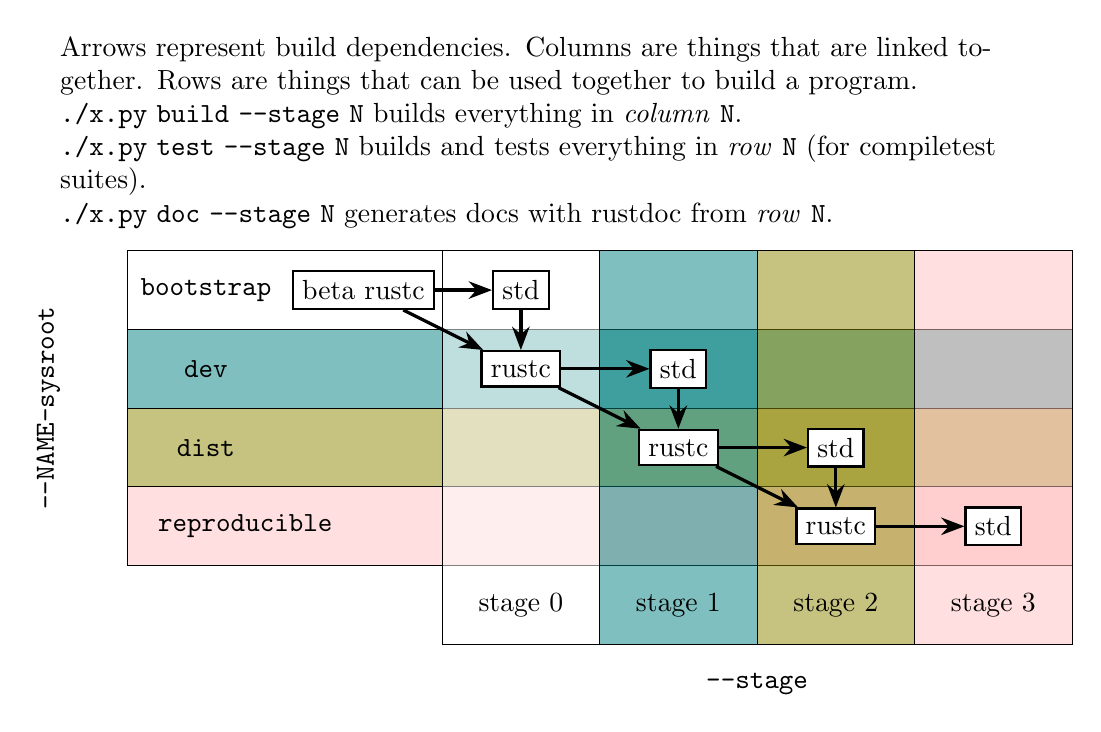
\begin{tikzpicture}
\node[text width=5in] at (2.5, 2) {
\noindent Arrows represent build dependencies.
Columns are things that are linked together.
Rows are things that can be used together to build a program.
\\
\noindent \verb|./x.py build --stage N| builds everything in \emph{column} \verb|N|.\\
\noindent \verb|./x.py test --stage N| builds and tests everything in \emph{row} \verb|N| (for compiletest suites).\\
\noindent \verb|./x.py doc --stage N| generates docs with rustdoc from \emph{row} \verb|N|.\\
};
\draw[draw=black,fill=white,fill opacity=0.5] (-3, -0.5) rectangle ++(12, 1);
\draw[fill=teal,fill opacity=0.5] (-3, -1.5) rectangle ++(12, 1);
\draw[fill=olive,fill opacity=0.5] (-3, -2.5) rectangle ++(12, 1);
\draw[fill=pink,fill opacity=0.5] (-3, -3.5) rectangle ++(12, 1);
\draw[draw=black,fill=white,fill opacity=0.5] (1, 0.5) rectangle ++(2, -5);
\draw[fill=teal,fill opacity=0.5] (3, 0.5) rectangle ++(2, -5);
\draw[fill=olive,fill opacity=0.5] (5, 0.5) rectangle ++(2, -5);
\draw[fill=pink,fill opacity=0.5] (7, 0.5) rectangle ++(2, -5);
\node[rotate=90] at (-4, -1.5) {\verb|--NAME-sysroot|};
\node[] at (-2, 0) {\verb|bootstrap|};
\node[] at (-2, -1) {\verb|dev|};
\node[] at (-2, -2) {\verb|dist|};
\node[] at (-1.5, -3) {\verb|reproducible|};
\node[] at (5, -5) {\verb|--stage|};
\node[] at (2, -4) {stage 0};
\node[] at (4, -4) {stage 1};
\node[] at (6, -4) {stage 2};
\node[] at (8, -4) {stage 3};
\begin{scope}[every node/.style={thick,draw,fill=white}]
	\node (s0r) at (0, 0) {beta rustc};
	\node (s0s) at (2,0) {std};
	\node (s1r) at (2,-1) {rustc};
	\node (s1s) at (4,-1) {std};
	\node (s2r) at (4,-2) {rustc};
	\node (s2s) at (6,-2) {std};
	\node (s3r) at (6,-3) {rustc};
	\node (s3s) at (8,-3) {std};
\end{scope}
\begin{scope}[>={Stealth[black]}, every edge/.style={draw=black,very thick}]
	\path [->] (s0r) edge node {} (s0s);
	\path [->] (s0r) edge node {} (s1r);
	\path [->] (s0s) edge node {} (s1r);
	\path [->] (s1r) edge node {} (s1s);
	\path [->] (s1r) edge node {} (s2r);
	\path [->] (s1s) edge node {} (s2r);
	\path [->] (s2r) edge node {} (s2s);
	\path [->] (s2r) edge node {} (s3r);
	\path [->] (s2s) edge node {} (s3r);
	\path [->] (s3r) edge node {} (s3s);
\end{scope}
\end{tikzpicture}
\end{document}
